% =========================
% Verifiable Counting in VLMs — Full Story + Detailed LaTeX Draft
% =========================
\documentclass[10pt]{article}

% ----- Packages -----
\usepackage[utf8]{inputenc}
\usepackage[T1]{fontenc}
\usepackage{times}
\usepackage{microtype}
\usepackage{graphicx}
\usepackage{subcaption}
\usepackage{booktabs}
\usepackage{multirow}
\usepackage{amsmath, amssymb}
\usepackage{siunitx}
\usepackage{hyperref}
\usepackage{xcolor}
\usepackage{enumitem}
\usepackage{cleveref}
\usepackage{xspace}

% ----- Macros -----
\newcommand{\dataset}{\textsc{SynthCount}\xspace}         % 400-image benchmark
\newcommand{\trainset}{\textsc{DetectCount-10k}\xspace}   % 10k finetune dataset

\newcommand{\gptfour}{\textsc{GPT-4o}\xspace}
\newcommand{\gptfive}{\textsc{GPT-5.2}\xspace}
\newcommand{\qwenbase}{\textsc{Qwen3-VL-2B}\xspace}
\newcommand{\qwenft}{\textsc{Qwen3-VL-2B + LoRA}\xspace}

\newcommand{\iou}{\ensuremath{\mathrm{IoU}}\xspace}
\newcommand{\fOne}{\ensuremath{\mathrm{F1}}\xspace}
\newcommand{\mae}{\ensuremath{\mathrm{MAE}}\xspace}

\newcommand{\visionstart}{\texttt{<|vision\_start|>}\xspace}
\newcommand{\visionend}{\texttt{<|vision\_end|>}\xspace}
\newcommand{\boxstart}{\texttt{<|box\_start|>}\xspace}
\newcommand{\boxend}{\texttt{<|box\_end|>}\xspace}
\newcommand{\objrefstart}{\texttt{<|object\_ref\_start|>}\xspace}
\newcommand{\objrefend}{\texttt{<|object\_ref\_end|>}\xspace}

\newcommand{\tauIoU}{0.5}

% ----- Title -----
\title{\vspace{-1.2em}
\textbf{Verifiable Counting in Vision--Language Models via Detection-as-Counting}\\
\vspace{-0.4em}\large From answer-only estimation to spatially grounded enumeration
\vspace{-0.8em}}
\author{Anonymous Authors}
\date{}

\begin{document}
\maketitle

% =========================
\begin{abstract}
Counting is a minimal primitive for visual reasoning and measurement, yet modern vision--language models (VLMs) often produce correct numbers for the wrong reasons---via estimation, shortcut cues, or ungrounded ``reasoning'' text.
We argue that dense counting should be evaluated as \emph{verifiable counting}, where the model must provide spatial evidence (e.g., bounding boxes for each instance) together with the final count.
We build a controlled synthetic benchmark \dataset with four difficulty tiers that systematically increase clutter, overlap, and distractors while preserving perfect instance-level ground truth.
Across closed- and open-source models, we observe near-perfect performance on small counts (subitizing) followed by catastrophic failure as density scales.
We then fine-tune \qwenbase with a Detection-as-Counting objective using \trainset, shifting outputs from hallucinated explanations to explicit spatial enumeration.
This yields large improvements on medium/hard tiers and dramatically reduces mean absolute error, but an \emph{alignment collapse} regime emerges at extreme density: the model continues emitting plausible box-format outputs while localization fidelity degrades.
Our results suggest that improving dense counting requires instance-level representations and/or higher-resolution visual processing beyond prompt engineering or decoder-only adaptation.
\end{abstract}

% =========================
\section{Introduction}
Counting is fundamental to real-world perception: it supports inventory, scene understanding, and measurement-like reasoning.
In embodied or physical contexts, counting often acts as a latent subroutine for higher-level tasks such as conservation, density estimation, and interaction planning.
However, counting differs from many VLM benchmarks in a key way: \emph{the answer is falsifiable}.
If a system claims there are 37 red squares, it should be able to point to those squares.

\paragraph{Problem.}
Current VLM evaluations typically treat counting as an answer-only task (output a single integer).
This setting conflates two distinct capabilities:
\begin{itemize}[leftmargin=1.2em]
  \item \textbf{Perceptual instance separation:} can the model represent \emph{individual} objects under clutter and occlusion?
  \item \textbf{Numeric reporting:} can the model map a set of perceived instances to an accurate integer?
\end{itemize}
Answer-only evaluation allows a model to ``pass'' by estimation or shortcut cues (e.g., approximate density).
Conversely, failures may stem from format, decoding, or miscalibration rather than perception.

\paragraph{Key hypothesis.}
We hypothesize that \emph{grounding-enabled} VLMs still lack \emph{instance-token disentanglement} required for stable counting.
Even if a model can follow prompts like ``locate the red car'' (referring grounding), this does not imply it can enumerate dozens of similar instances.
Thus, dense counting failure may reflect a representational bottleneck: patch-based encoders and global pooled features are insufficient to maintain distinct instance identities when targets are dense and overlapping.

\paragraph{Our approach: verifiable counting.}
We propose to evaluate counting with \emph{spatial evidence}, requiring bounding boxes for each detected target instance before reporting the final count.
This makes counting outcomes auditable and separates \emph{format compliance} from \emph{true spatial grounding}.

\paragraph{Contributions.}
\begin{itemize}[leftmargin=1.2em]
  \item \textbf{Controlled benchmark (\dataset).} A tiered synthetic counting dataset (400 images) with perfect instance-level boxes, designed to probe failure as clutter/distractors/occlusion scale.
  \item \textbf{SOTA diagnostic.} A direct comparison on matched samples showing strong subitizing but catastrophic breakdown at scale for \gptfour, \gptfive, and \qwenbase.
  \item \textbf{Detection-as-Counting fine-tuning.} A 10k multimodal training set (\trainset) and LoRA adaptation that shifts \qwenbase from hallucinated ``analysis'' to explicit enumeration.
  \item \textbf{Grounding fidelity analysis.} IoU-based matching shows that even when counting improves, localization degrades sharply at extreme density, revealing an \emph{alignment collapse} regime.
\end{itemize}

% =========================
\section{Related Work}
\subsection{Visual Counting and Numerosity}
Classic counting work distinguishes subitizing (small counts, near-instant) from approximate numerosity estimation (larger counts).
In dense scenes, occlusion and overlap introduce the core difficulty: the system must separate instances and avoid double-counting.
Prior datasets often mix counting with semantics (e.g., natural images), making it hard to attribute errors to perception vs.\ recognition.
\textbf{Our focus is diagnostic control:} we deliberately remove semantic confusion (simple shapes) to isolate the instance separation problem.

\subsection{Grounding and Referring Expression in VLMs}
Many VLMs support grounding by representing bounding boxes as text tokens.
For example, inputs may include \visionstart \dots \visionend and outputs may include \boxstart \dots \boxend linked via \objrefstart \dots \objrefend.
This mechanism enables referring-grounding and region description, but it does not guarantee that internal vision representations form stable, distinct instance tokens when asked to enumerate many objects.
\textbf{Our paper tests exactly this gap:} grounding tokens exist, but counting still fails at scale.

\subsection{Instance-level Representations and Dense Region Features}
Object-centric models (e.g., query-based detectors, slot attention, object proposals) explicitly represent scenes as a set of instance slots.
In contrast, ViT-style patch tokens often serve as a dense grid without explicit object identity.
Recent work explores region-level contrastive models (dense CLIP variants) and distillation from detectors to produce localized features.
\textbf{Our method is a lightweight step:} we do not replace the encoder; instead we test whether a verifiable supervision signal can reshape a VLM toward instance-like enumeration, and we characterize where this fails.

% =========================
\section{Benchmark: \dataset}
\subsection{Design Goals}
We design \dataset to satisfy four goals:
\begin{enumerate}[leftmargin=1.2em]
  \item \textbf{Controlled difficulty.} We vary density, overlap, background complexity, and distractors in a principled way.
  \item \textbf{Perfect ground truth.} Each object has exact bounding-box supervision, enabling precise grounding evaluation.
  \item \textbf{Minimal semantics.} Shapes/colors prevent semantic recognition from dominating; the primary challenge is instance separation.
  \item \textbf{Stress-test scaling.} We include an Extreme tier (51--100 objects) to probe resolution limits and failure modes.
\end{enumerate}

\subsection{Generation Pipeline}
We implement a Pillow-based renderer that procedurally samples:
\begin{itemize}[leftmargin=1.2em]
  \item \textbf{Targets:} colored geometric shapes with controlled size distribution.
  \item \textbf{Distractors:} non-target shapes and colors, capped by tier.
  \item \textbf{Backgrounds:} from uniform to textured/complex as tier increases.
  \item \textbf{Placement:} increasing overlap/occlusion as tier increases.
\end{itemize}
We generate 400 images total (100 per tier) and store per-image annotations: target class, list of target boxes, list of distractor boxes (optional), and the true count.

\subsection{Difficulty Tiers}
\begin{itemize}[leftmargin=1.2em]
  \item \textbf{Easy:} 1--5 objects; clean background; no overlap; no distractors.
  \item \textbf{Medium:} 6--20 objects; colored background; partial overlap; up to 5 distractors.
  \item \textbf{Hard:} 21--50 objects; complex background; significant overlap; up to 15 distractors.
  \item \textbf{Extreme:} 51--100 objects; high density; heavy occlusion; up to 25 distractors.
\end{itemize}

\subsection{Protocols: Count-only vs.\ Verifiable Counting}
\paragraph{Count-only.}
We query: ``How many \emph{target} objects are in the image? Output an integer only.''
This isolates raw numeric performance but is vulnerable to estimation.

\paragraph{Verifiable counting.}
We query: ``Annotate each target object with a bounding box, then state \texttt{Total count: N}.''  
This enforces an explicit enumeration trace that can be checked against ground truth, enabling a \emph{verifiability} lens:
even when the final number is correct, the model may be wrong about \emph{which} objects it counted.

% =========================
\section{Models and Evaluation}
\subsection{Models}
We evaluate:
\begin{itemize}[leftmargin=1.2em]
  \item \textbf{Closed-source:} \gptfour and \gptfive on a matched 80-image subset (20 per tier), using the same prompt and decoding constraints.
  \item \textbf{Open-source:} \qwenbase as the baseline VLM.
  \item \textbf{Fine-tuned:} \qwenft trained with Detection-as-Counting on \trainset and merged for inference.
\end{itemize}

\subsection{Metrics}
\paragraph{Counting.}
Exact-match accuracy and mean absolute error:
\[
\mae = \frac{1}{N}\sum_{i=1}^{N} \left| \hat{c}_i - c_i \right|.
\]

\paragraph{Grounding fidelity (IoU matching).}
For each image, we match predicted boxes to ground-truth target boxes with a greedy bipartite procedure:
a prediction is a true positive if it matches an \emph{unused} ground-truth box with $\iou \ge \tau$, where $\tau = \tauIoU$.
We compute precision/recall/\fOne per image and average within each tier.

\paragraph{Why we need both.}
Counting accuracy alone can be misleading: a model may output the correct count by accident, estimation, or compensating errors (missing some objects but double-counting others).
Grounding metrics reveal whether the model truly identifies the correct instances.

% =========================
\section{SOTA Diagnostic: Counting Fails at Scale}
\subsection{Closed-source: \gptfour vs.\ \gptfive}
We observe a clear pattern:
\textbf{subitizing works}, moderate clutter is partially solvable, and dense scenes induce catastrophic failure.
Notably, \gptfive improves significantly on Medium, suggesting better selective attention in moderately cluttered scenes, but both models fail on Extreme.

\begin{table}[t]
  \centering
  \small
  \setlength{\tabcolsep}{6pt}
  \begin{tabular}{lcccc}
    \toprule
    \multirow{2}{*}{\textbf{Tier}} & \multicolumn{2}{c}{\textbf{Accuracy (\%)}} & \multicolumn{2}{c}{\textbf{\mae}} \\
    \cmidrule(lr){2-3}\cmidrule(lr){4-5}
     & \gptfour & \gptfive & \gptfour & \gptfive \\
    \midrule
    Easy     & 100.0 & 95.0  & 0.00 & 0.05 \\
    Medium   & 20.0  & 65.0  & 1.20 & 0.35 \\
    Hard     & 5.0   & 10.0  & 4.45 & 3.40 \\
    Extreme  & 0.0   & 0.0   & 10.65 & 9.95 \\
    \bottomrule
  \end{tabular}
  \caption{Closed-source models on the same 80 images. Both models fail on dense scenes; \gptfive improves in Medium but does not solve Hard/Extreme.}
  \label{tab:sota_counting}
\end{table}

\subsection{Open-source baseline: \qwenbase}
We evaluate \qwenbase on 200 images (random subset) and see severe degradation beyond Easy.
This establishes that counting is not a native strength of the model despite general grounding capabilities.

\begin{table}[t]
  \centering
  \small
  \setlength{\tabcolsep}{6pt}
  \begin{tabular}{lcc}
    \toprule
    \textbf{Tier} & \textbf{Accuracy (\%)} & \textbf{\mae} \\
    \midrule
    Easy     & 95.5 & 0.05 \\
    Medium   & 14.6 & 14.69 \\
    Hard     & 1.8  & 24.95 \\
    Extreme  & 0.0  & 67.27 \\
    \midrule
    Overall  & 25.0 & 28.01 \\
    \bottomrule
  \end{tabular}
  \caption{\qwenbase collapses under clutter/density; Extreme is catastrophic.}
  \label{tab:qwen_base}
\end{table}

\paragraph{Qualitative observation: ``hallucinated enumeration.''}
On moderately dense scenes, the baseline model often produces verbose step-by-step text that repeatedly mentions the same region/shape, sometimes failing to output the final integer at all (e.g., looping until the token limit).
This motivates enforcing a strict verifiable output format.

% =========================
\section{Prompting Intervention: Visual Chain-of-Thought (vCoT)}
We test whether forcing intermediate spatial reporting improves counting without changing weights.
The vCoT prompt requests approximate coordinates for each detected instance before providing the final count.
This improves Medium performance, suggesting that explicit grounding can help attention allocation, but the effect saturates and does not solve Extreme.

\begin{table}[t]
  \centering
  \small
  \setlength{\tabcolsep}{6pt}
  \begin{tabular}{lcccc}
    \toprule
    \multirow{2}{*}{\textbf{Tier}} & \multicolumn{2}{c}{\textbf{Accuracy (\%)}} & \multicolumn{2}{c}{\textbf{\mae}} \\
    \cmidrule(lr){2-3}\cmidrule(lr){4-5}
     & Baseline & vCoT & Baseline & vCoT \\
    \midrule
    Easy     & 95.0 & 100.0 & 0.05 & 0.00 \\
    Medium   & 65.0 & 80.0  & 0.35 & 0.20 \\
    Hard     & 10.0 & 15.0  & 3.40 & 2.55 \\
    Extreme  & 0.0  & 0.0   & 9.95 & 9.85 \\
    \bottomrule
  \end{tabular}
  \caption{vCoT helps Medium but does not break the dense counting barrier.}
  \label{tab:vcot}
\end{table}

\paragraph{Interpretation: the attention ceiling.}
vCoT provides more test-time structure, but the model still cannot reliably maintain distinct instances under high density.
This supports the view that dense counting requires representational changes (instance-level tokens or higher-resolution processing), not just prompting.

% =========================
\section{Method: Detection-as-Counting Fine-tuning}
\subsection{Training Data: \trainset}
We build \trainset (10,000 samples) by pairing images with a strict response template:
the assistant must output one bounding box per target instance, then output \texttt{Total count: N}.
Boxes are normalized to a consistent coordinate system and expressed as text tokens delimited by \boxstart and \boxend.
This format aligns with grounding token conventions used by grounding-enabled VLMs.

\subsection{Fine-tuning Setup}
We fine-tune \qwenbase using LoRA in LLaMA-Factory.
We target:
\begin{itemize}[leftmargin=1.2em]
  \item \textbf{Decoder attention projections} (e.g., \texttt{q\_proj}, \texttt{v\_proj}) to adapt generation dynamics toward enumeration.
  \item \textbf{Vision-language interface layers} (e.g., \texttt{vision\_embed\_tokens}) to better align visual features with box-text emission.
\end{itemize}
The objective is standard supervised fine-tuning (teacher forcing) over the box sequence and the final count.

\subsection{Counting Results}
\begin{table}[t]
  \centering
  \small
  \setlength{\tabcolsep}{6pt}
  \begin{tabular}{lcccc}
    \toprule
    \multirow{2}{*}{\textbf{Tier}} & \multicolumn{2}{c}{\textbf{Accuracy (\%)}} & \multicolumn{2}{c}{\textbf{\mae}} \\
    \cmidrule(lr){2-3}\cmidrule(lr){4-5}
     & Base & Fine-tuned & Base & Fine-tuned \\
    \midrule
    Easy     & 95.5 & 93.2 & 0.05 & 0.07 \\
    Medium   & 14.6 & 58.3 & 14.69 & 0.52 \\
    Hard     & 1.8  & 12.5 & 24.95 & 2.82 \\
    Extreme  & 0.0  & 0.0  & 67.27 & 9.96 \\
    \bottomrule
  \end{tabular}
  \caption{Detection-as-Counting fine-tuning: major MAE reduction and improved accuracy on Medium/Hard, but Extreme remains unsolved.}
  \label{tab:finetune_count}
\end{table}

\paragraph{What changed qualitatively.}
Fine-tuning reliably eliminates hallucinated long-form ``analysis'' outputs and replaces them with strict enumeration:
a sequence of box tokens followed by a single numeric statement.
This is a \emph{behavioral phase shift} from estimation to verifiable output, enabling systematic auditing.

% =========================
\section{Grounding Fidelity: IoU Matching and Alignment Collapse}
\subsection{Why grounding fidelity matters}
A model can learn to output the \emph{format} of a box list without actually grounding boxes to the correct pixels.
Therefore, we verify whether predicted boxes correspond to ground truth using \iou matching.

\subsection{IoU@$\tau$ Evaluation}
We use $\tau=\tauIoU$.
Precision answers: \emph{Are predicted boxes objects (and correct targets)?}
Recall answers: \emph{Did the model find all target instances?}
We report per-tier averages.

\begin{table}[t]
  \centering
  \small
  \setlength{\tabcolsep}{6pt}
  \begin{tabular}{lccc}
    \toprule
    \textbf{Tier} & \textbf{Precision (\%)} & \textbf{Recall (\%)} & \textbf{\fOne (\%)} \\
    \midrule
    Easy     & 95.15 & 98.18 & 96.51 \\
    Medium   & 93.61 & 93.98 & 93.68 \\
    Hard     & 85.11 & 87.97 & 86.46 \\
    Extreme  & 58.61 & 55.99 & 56.98 \\
    \midrule
    Overall  & 83.34 & 84.22 & 83.62 \\
    \bottomrule
  \end{tabular}
  \caption{Grounding fidelity (IoU@0.5). Extreme shows severe degradation despite format compliance.}
  \label{tab:iou}
\end{table}

\subsection{Qualitative analysis: ``Alignment collapse''}
To make the difficulty progression explicit, \cref{fig:tier_examples} shows one representative raw input from each tier.
From Easy to Extreme, object count, clutter, overlap, and distractors all increase.

\begin{figure}[t]
  \centering
  \begin{subfigure}[b]{0.48\linewidth}
    \centering
    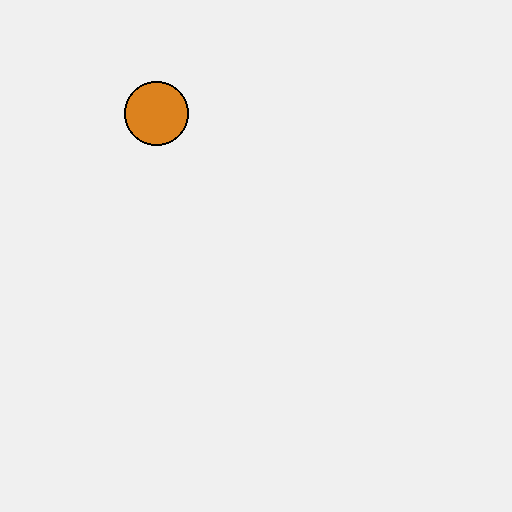
\includegraphics[width=\linewidth]{figures/example_easy.png}
    \caption{Easy (1--5 objects).}
    \label{fig:example_easy}
  \end{subfigure}
  \hfill
  \begin{subfigure}[b]{0.48\linewidth}
    \centering
    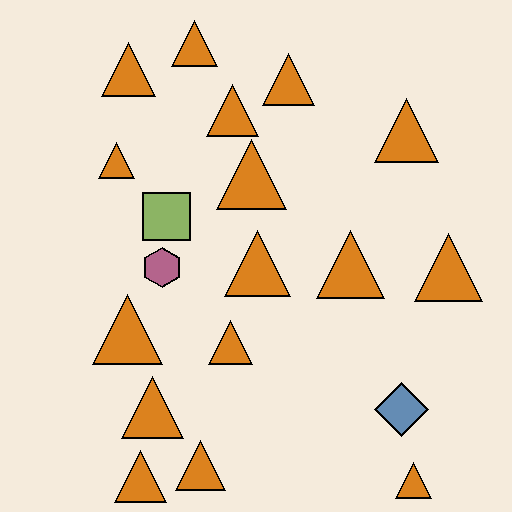
\includegraphics[width=\linewidth]{figures/example_medium.png}
    \caption{Medium (6--20 objects).}
    \label{fig:example_medium}
  \end{subfigure}

  \vspace{0.5em}

  \begin{subfigure}[b]{0.48\linewidth}
    \centering
    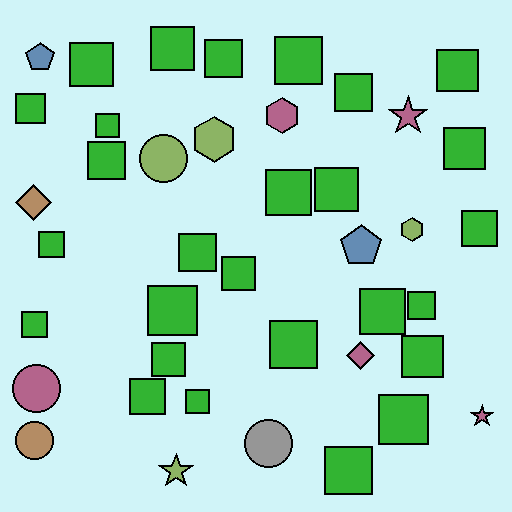
\includegraphics[width=\linewidth]{figures/example_hard.png}
    \caption{Hard (21--50 objects).}
    \label{fig:example_hard}
  \end{subfigure}
  \hfill
  \begin{subfigure}[b]{0.48\linewidth}
    \centering
    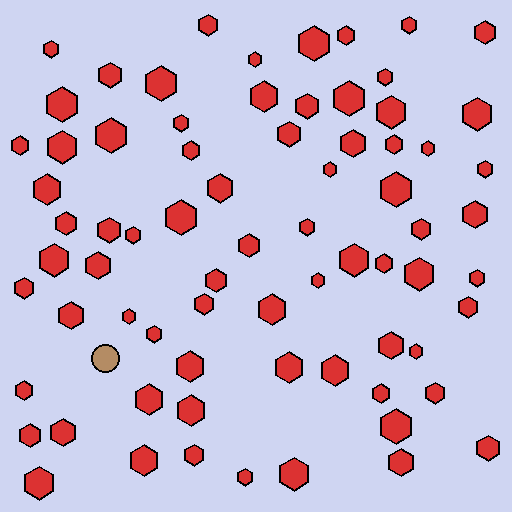
\includegraphics[width=\linewidth]{figures/example_extreme.png}
    \caption{Extreme (51--100 objects).}
    \label{fig:example_extreme}
  \end{subfigure}
  \caption{Representative inputs from \dataset across difficulty tiers.}
  \label{fig:tier_examples}
\end{figure}

We then visualize predicted boxes (red) vs.\ ground truth (green) on challenging cases in \cref{fig:qual} and observe a consistent transition:
\begin{itemize}[leftmargin=1.2em]
  \item \textbf{Easy/Medium (typically):} localization is usually tight and distractors are mostly excluded.
  \item \textbf{Hard:} increasing duplicate jitter (multiple boxes per object), merge boxes (one box covers several adjacent objects), and missed dense clusters.
  \item \textbf{Extreme:} chaotic boxing behavior: oversized enclosures, distractor capture, empty-space boxing, and systematic misses in crowded regions.
\end{itemize}
Crucially, the model can sometimes output a numerically close count while spatial evidence is incorrect.
This explains why count-only metrics can overestimate true counting ability.

\begin{figure}[t]
  \centering
  \begin{subfigure}[b]{0.48\linewidth}
    \centering
    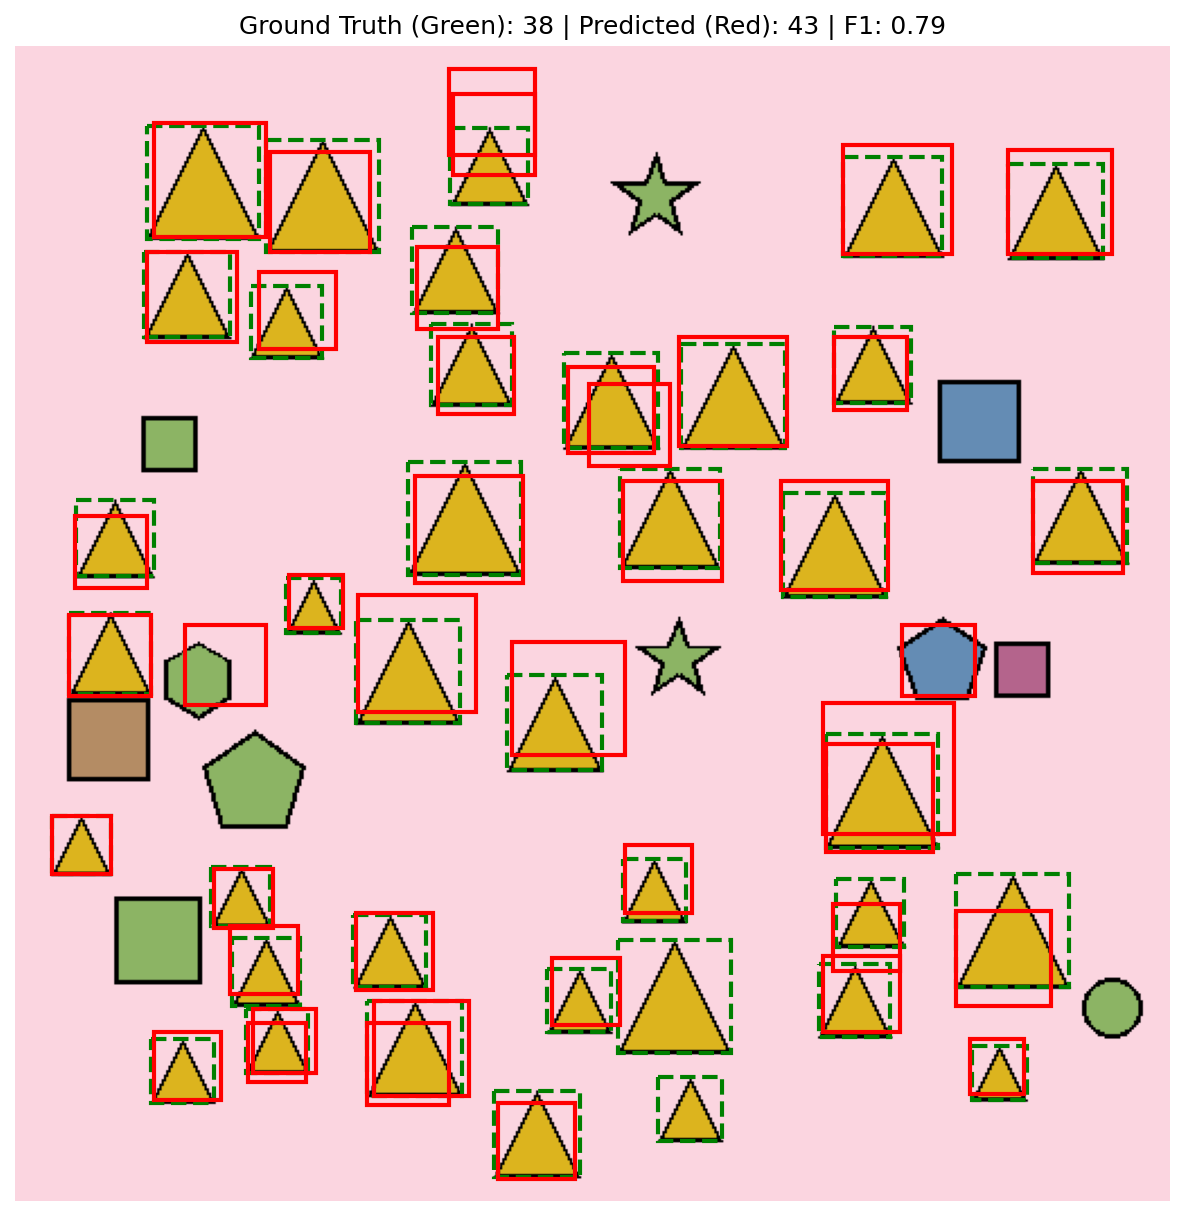
\includegraphics[width=\linewidth]{figures/pred_hard_3.png}
    \caption{Hard case A: duplicate and merged boxes.}
    \label{fig:hard3}
  \end{subfigure}
  \hfill
  \begin{subfigure}[b]{0.48\linewidth}
    \centering
    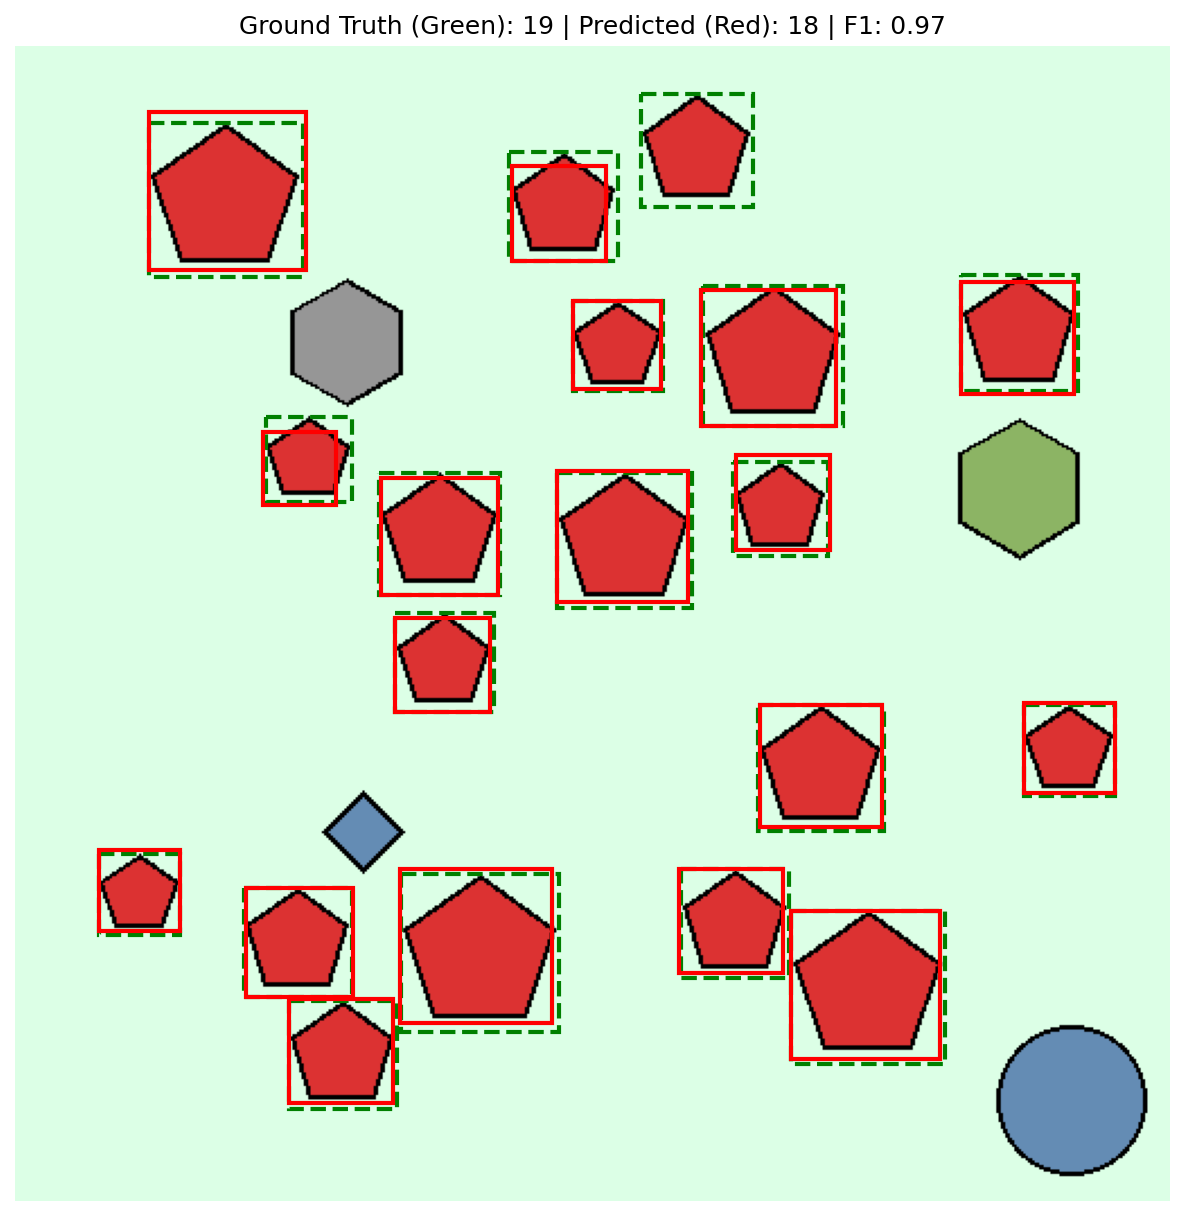
\includegraphics[width=\linewidth]{figures/pred_hard_4.png}
    \caption{Hard case B: misses in dense clusters.}
    \label{fig:hard4}
  \end{subfigure}

  \vspace{0.6em}

  \begin{subfigure}[b]{0.48\linewidth}
    \centering
    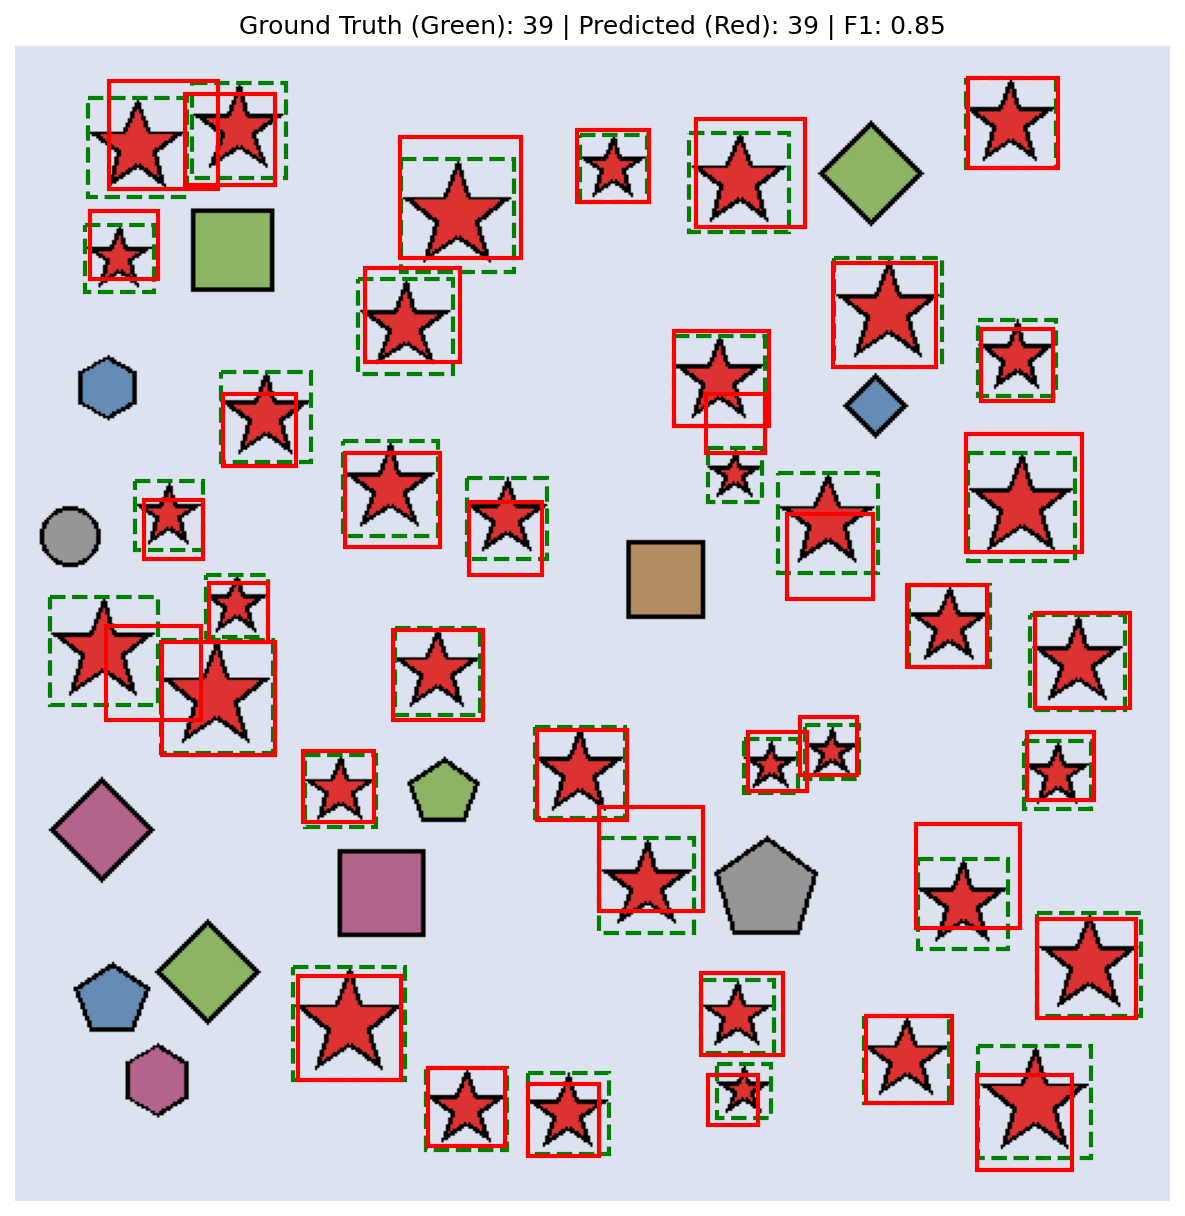
\includegraphics[width=\linewidth]{figures/pred_extreme_5.png}
    \caption{Extreme case A: oversized boxes and confusion.}
    \label{fig:hard5}
  \end{subfigure}
  \hfill
  \begin{subfigure}[b]{0.48\linewidth}
    \centering
    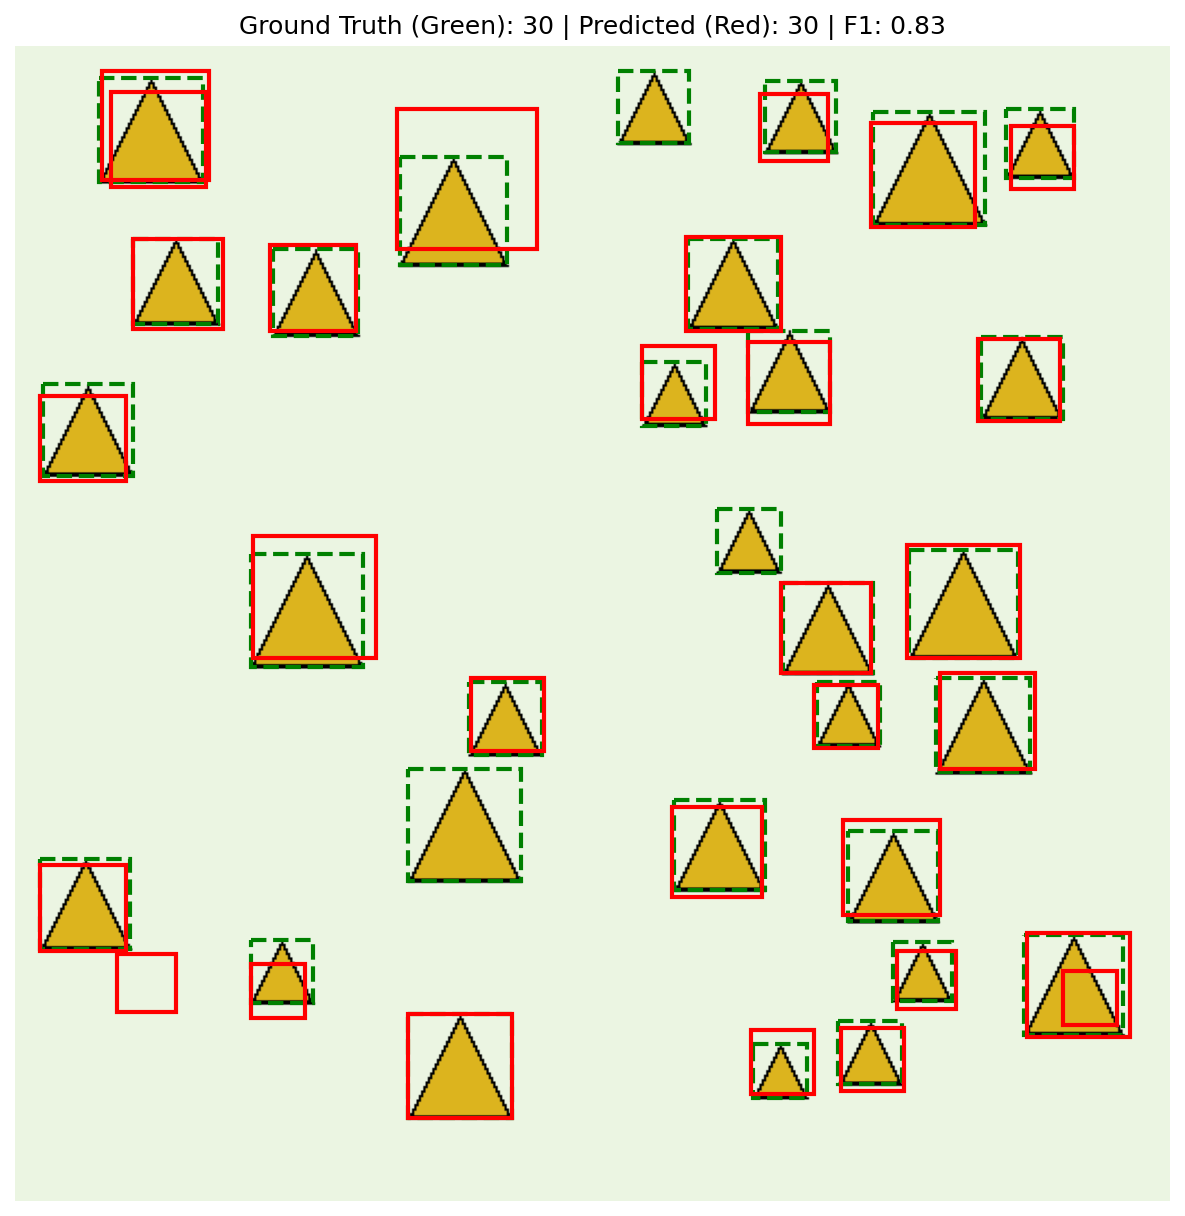
\includegraphics[width=\linewidth]{figures/pred_extreme_13.png}
    \caption{Extreme case B: distractor capture and empty-space boxing.}
    \label{fig:hard13}
  \end{subfigure}
  \caption{Marked predictions (red) vs.\ ground truth (green) on Hard/Extreme images. ``Alignment collapse'' emerges as density increases.}
  \label{fig:qual}
\end{figure}

% =========================
\section{Discussion}
\subsection{What did we learn?}
Our results support three claims:
\begin{enumerate}[leftmargin=1.2em]
  \item \textbf{Dense counting is unresolved.} Even strong models fail when scenes exceed moderate density and include distractors/occlusion.
  \item \textbf{Prompting helps but saturates.} vCoT improves Medium but does not solve Extreme, indicating limitations in internal representations.
  \item \textbf{Verifiable supervision shifts behavior.} Detection-as-Counting fine-tuning dramatically reduces \mae and improves accuracy for Medium/Hard, and it turns hallucinated explanations into auditable enumerations.
\end{enumerate}

\subsection{Why does Extreme remain unsolved?}
The persistence of failure at Extreme suggests a \textbf{representation bottleneck}:
\begin{itemize}[leftmargin=1.2em]
  \item Patch-based encoders may not preserve enough spatial resolution to separate adjacent instances.
  \item Dense overlap causes multiple objects to share similar patch evidence, leading to merges and misses.
  \item Decoder adaptation alone cannot create instance tokens if the encoder collapses them.
\end{itemize}
This motivates architectural interventions rather than only supervision or prompting.

\subsection{A practical ``verifiability'' perspective}
Even if a model cannot perfectly count 100 objects, verifiable outputs provide \emph{diagnostic and product value}:
downstream systems can reject low-fidelity enumerations, request zoomed crops, or trigger tool use.
Thus, the evaluation framework and failure analysis are useful even before perfect solving.

% =========================
\section{Future Work}
We outline three concrete next steps that strengthen publishability:
\subsection{High-resolution tiling and merge}
Split the image into overlapping tiles, run enumeration per tile, and merge boxes across tiles via NMS-like matching.
This directly addresses the patch-resolution bottleneck without retraining the encoder.

\subsection{Instance-token adapter (parallel head)}
Add a lightweight object-query module (e.g., DETR-like queries or slot attention) that produces $K$ instance slots from vision tokens, then condition the LLM decoder on these slots.
This creates explicit instance tokens while reusing the existing VLM backbone.

\subsection{Distillation from a detector or dense region teacher}
Use an external detector (or dense region model) as a teacher and distill instance-level supervision into the vision encoder or adapter.
This is aligned with your earlier direction: dense CLIP / crop-CLIP / teacher distillation to induce localized, instance-aware embeddings.

% =========================
\section{Limitations}
\begin{itemize}[leftmargin=1.2em]
  \item \textbf{Synthetic-to-real gap:} shapes differ from natural scenes; however, synthetic control isolates the counting bottleneck cleanly.
  \item \textbf{Evaluation scope:} we tested representative subsets; scaling evaluation to more models and larger samples would strengthen claims.
  \item \textbf{Architecture inference:} we attribute Extreme failure partly to resolution limits; confirming this requires controlled patch-size or multi-scale encoder experiments.
\end{itemize}

% =========================
\section{Conclusion}
We propose \emph{verifiable counting} as a diagnostic and evaluation framework for VLMs.
Across closed- and open-source models, we find strong performance in low-count settings but catastrophic failure as density and distractors scale.
Detection-as-Counting fine-tuning shifts open-source VLM behavior from hallucinated explanation to auditable spatial enumeration and yields large gains in Medium/Hard tiers.
However, IoU-based analysis reveals an alignment collapse regime at Extreme density, indicating that solving dense counting likely requires instance-level representations and/or higher-resolution visual processing.
Our benchmark, evaluation protocol, and analyses provide a concrete roadmap for future instance-aware VLM research.

% =========================
% Bibliography placeholder
% =========================
% \bibliographystyle{plain}
% \bibliography{refs}

\end{document}
